
\subsection{Módulo de procesamiento de medidas}
% ----------------------------------------------------------------------
% D- Módulo de estimación de la trayectoria
% - Objetivo del módulo	
El objetivo de este módulo es proveer al usuario algoritmos básicos para la localización a partir de las señales generadas. Estos algoritmos se utilizarán como punto de partida para el diseño de nuevos. 

% - Interfaz de los algoritmos de localización
En Navindoor se encuentra implementados  el filtro de Kalman extendido (EKF)\cite{Kay:1993:FSS:151045} y el Filtro de Kalman \emph{Unscented} (UKF) \cite{UKF}. Para implementar nuevos algoritmos es necesario que estos tengan una interfaz de entrada/salida específica. Los algoritmos deberán tener tres parámetros de entrada: El objeto \emph{building}, una lista de las señales generadas en todos los instantes de tiempo y una estructura con toda la información a \emph{priori} de la trayectoria. Además deberán tener como parámetro de salida una matriz de cuatro columnas. Las tres primeras columnas indicando el espacio y la última columna el tiempo (figura \ref{format}). Navindoor se encarga de procesar esta información para crear un objeto trayectoria. De esta manera la estimación contará con las propiedades y métodos de la trayectoria real.  
\begin{figure}[ht!]
    \centering
        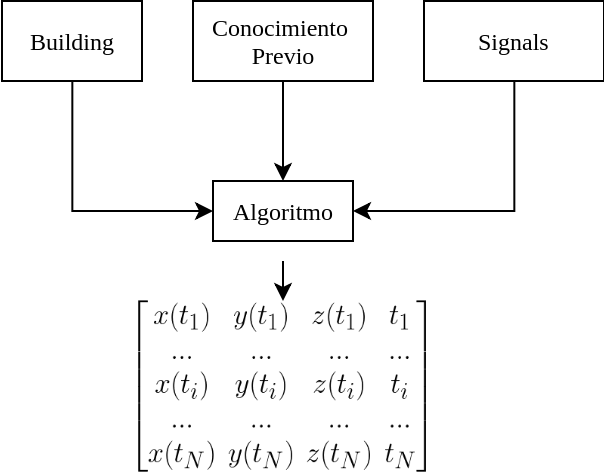
\includegraphics[width=0.725\columnwidth]{img/Design/InterfazAlgo.png}
        \caption{Interfaz de entrada/salida para los algoritmos de localización}
        \footnotesize
        Como entrada tiene tres variables, la primera representando la planimetría, la segunda representado todo el conocimiento previo sobre la trayectoria y el tercero un listado de las señales. El algoritmo devuelve una matriz $4 \times N$, siendo N el número de medidas
        \label{format}
    \end{figure}

% - Explicación básica del procesado de medidas y estimación de la trayectoria
Con respecto a la GUI, Navindoor muestra un listado de las trayectorias que han sido generadas. Para cada una de estas trayectorias podemos ver las señales disponibles. De esta manera podemos seleccionar la trayectoria y las señales que queramos procesar. Dado que los algoritmos tienen el interfaz entrada/salida antes presentado, es posible ejecutarlos con un solo \emph{click}. Navindoor, luego de ejecutar el algoritmo muestra la trayectoria real y la trayectoria estimada dentro de la planimetría cargada. Además gracias a que la estimación es un objeto trayectoria, podemos utilizar la animación utilizada en el módulo de generación de trayectorias, dando una visión a tiempo real del comportamiento de la trayectoria real frente a la trayectoria estimada.